\documentclass[]{beamer}

\usepackage[T1]{fontenc}
\usepackage[utf8]{inputenc}
\usepackage{booktabs}
\usepackage{relsize}
\usepackage{graphicx}
\usepackage{amssymb,amsmath,amsfonts,amsthm}

\addtobeamertemplate{navigation symbols}{}{%
    \usebeamerfont{footline}%
    \usebeamercolor[fg]{footline}%
    \hspace{1em}%
    \larger%
    \insertframenumber/\inserttotalframenumber
}
\def\fm#1{\text{\texttt{#1}}} % use ams
\def\energy{E}
\def\coat{\fm{CoAT}}
\def\sim{\sigma}
\def\modeleXFun{\mathcal{S}}
\def\modeleYFun{\mathcal{R}}
\def\simS{\sim_\modeleXFun}
\def\simR{\sim_\modeleYFun}
\def\source{s}
\def\cible{t}
\def\case{c}
\def\outcome{r}
\def\outcomes{\mathcal{R}}
\def\ts{\mathcal{T}}
\def\card#1{\vert#1\vert}
\def\donne{\longrightarrow}
\def\potential#1{\hat{#1}}
\def\ensS{\mathcal{S}}
\def\ensO{\mathcal{R}}
\def\ensX{\mathcal{X}}
\def\ensY{\mathcal{Y}}
\DeclareMathOperator*{\argmin}{arg\,min}
\DeclareMathOperator*{\argmax}{arg\,max}
\DeclareMathOperator*{\minimum}{min}
\DeclareMathOperator*{\maximum}{max}
\newcommand{\norm}[1]{\left\lVert#1\right\rVert_{2}}
\newcommand\given[1][]{\:#1\vert\:}
\def\x{\textbf{x}}
\def\y{\textbf{y}}
\def\Reels{\mathbb{R}}
\def\transpose{^{T}}
\newcommand\telque[1][]{\:#1\vert\:}
\def\card#1{\vert#1\vert}

\title{Maintenance benchmark on real world data 2}
\author{Esteban Marquer}
\date{6 november}

\begin{document}

\begin{frame}
    \titlepage
\end{frame}
% \section{Baseline}
% \begin{frame}{Goal}
%     \begin{enumerate}
%         \item Get a results on real data
%         \item Get a benchmark on real data for CB maintenance\\
%         $\rightarrow$ Reproduce the setting from:\\

%         ``Combining and Choosing Case Base Maintenance Algorithms''
%         Ph.D. thesis of Lisa Cummins, 2013
%     \end{enumerate}
    

%\end{frame}
\begin{frame}
    \tableofcontents
\end{frame}
\begin{frame}{Baselines ~~{\smaller {\color{green!50!black}Green: maintenance baseline avail.}~~{\color{red} Red: not found}}}
    \begin{center}
        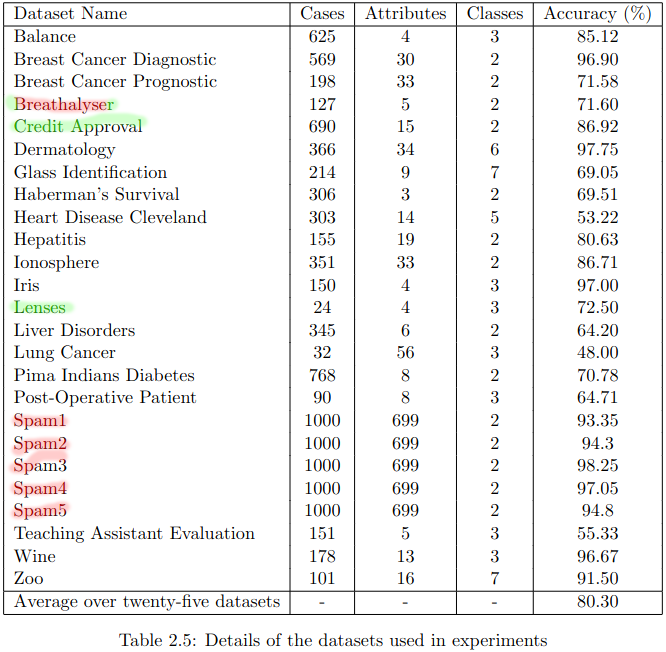
\includegraphics[width=.85\textwidth]{tab2_5_.png}
    \end{center}
    
\end{frame}
% \begin{frame}{Baselines maintainance}
%     \begin{center}
%         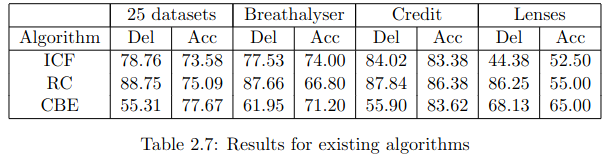
\includegraphics[width=.9\textwidth]{tab2_7.png}
%     \end{center}
    
%     \begin{itemize}
%         \item ICF:  Iterative Case Filtering [9]\\
%         {\smaller H. Brighton and C. Mellish. ``On the consistency of information filters for lazy learning algorithms'', 1999}
%         \item RC:  RC-CNN [58]\\
%         {\smaller E. McKenna and B. Smyth. ``Competence-guided case-base editing techniques'', 2000}
%         \item CBE (Case Base Editing) = BBNR (Blame-Based Noise Reduction) + CRR (Conservative Redundancy Reduction) [19]\\
%         {\smaller S.J. Delany and P. Cunningham. ``An analysis of case-based editing in a spam filtering system'', 2004.}
%     \end{itemize}

%     We copy these values for our baseline.
% \end{frame}
\begin{frame}{Current datasets}
    \centering
    \smaller
    \begin{tabular}{lrr}
        \toprule
        verbose name & found & has maintenance baseline \\\midrule
        \textbf{Lenses} & True & \textbf{True} \\
        \textbf{Credit Approval} & True & \textbf{True} \\
        Zoo & True & False \\
        Wine & True & False \\
        Teaching Assistant Evaluation & True & False \\
        Post-Operative Patient & True & False \\
        Pima indians Diabetes & True & False \\
        Lung Cancer & True & False \\
        Liver Disorders & True & False \\
        Iris & True & False \\
        Ionosphere & True & False \\
        Hepatitis & True & False \\
        Heart Disease Cleveland & True & False \\
        Haberman's Survival & True & False \\
        Glass Identification & True & False \\
        Dermatology & True & False \\
        Breast Cancer Pronostic & True & False \\
        Breast Cancer Diagnostic & True & False \\
        Balance & True & False \\\bottomrule
    \end{tabular}
\end{frame}
% \begin{frame}{Current datasets}
%     \centering
%     \begin{tabular}{lrr}
%         \toprule
%         verbose name & found & has maintenance baseline \\\midrule
%         \textbf{Breathalyser} & False & \textbf{True} \\
%         Spam5 & False & False \\
%         Spam4 & False & False \\
%         Spam3 & False & False \\
%         Spam2 & False & False \\
%         Spam1 & False & False \\\bottomrule
%     \end{tabular}
% \end{frame}

\section{Benchmark experiment setup}
\begin{frame}{Process}

    train/dev/test split: 60\%/20\%/20\%, as in the thesis

    ~

    train: cases in the CB at the start

    dev: cases used for maintenance decision

    test: cases used to mesure performance
    
\end{frame}
\begin{frame}{Similarity}

    \textbf{Numeric attribute:} $1 -$ normalized absolute distance
    $$sim(x,y) = 1 - \frac{x-y}{max(X) - min(X)}$$
    with $x,y$ the value of the att. for 2 cases,\\
    $X$ the values of the att. for all cases in the CB
    \\[2em]

    \textbf{Symbolic attribute:}
    $$sim(x,y) = 1 \text{ if } x=y \text{ else } 0$$
    with $x,y$ the value of the att. for 2 cases
    \\[2em]

    \textbf{Overall similarity:}
    weighted similarity (Karabulut \textit{et al.}, 2019)\footnote{\textit{``Weighted Similarity Measure for k-Nearest Neighbors Algorithm''}
    B. Karabulut, G. Arslan, H. M. Ünver, 2019, Celal Bayar University Journal of Science
}%(how the weights are obtained not mentioned in the thesis)

\end{frame}
\begin{frame}{Weight computation}
    \smaller
    $C_i(a)$: set of values for attribute $a$ belonging to class $i$
    $$C_i(a) = \{X[k][a]: X[k] \in X \text{ and }y[k]=i\}$$
    
~

    $A_i(a)$: set of cases with attribute $a$ within values of class $i$
    $$A_i(a) = \{X[k] \in X: min(C_i(a)) \leq X[k][a] \leq max(C_i(a))\}$$
    $$A_i(a) = \{X[k] \in X: X[k][a] \in C_i(a)\} \text{ for nominal att. (defined by me)}$$
    
~

    $B_i(a)$: set of cases with attribute $a$ within values of class $i$ but not any other class
    $$B_i(a) = A_i(a) - \cup_{i\ne j, j\in classes} A_j(a)$$
    
~

    $w_a$: weight for attribute $a$, average ``ability to discriminate''
    $$w_a=|\cup_{i\in classes} B_i(a)| / n, \; n: len(X)$$ 
    
    $w_a*=w_a/(\sum_{a'} w_{a'})$: normalized $w_a$

    ~

    {\smaller\smaller(in paper it was $w_a=(\bigcup_{i\in classes} |B_i(a)|) / n$, but it makes no sense)}

\end{frame}
% \begin{frame}{Attempt to fix weights}
%     Karabulut \textit{et al.}'s method not perfect

%     ~

%     Issue: may not scale well for symbolic attributes, as this part is custom made by me

%     ~

%     balance+scale: all $B_i(a)=\emptyset$, need to add a default value and weights end up all equal
% \end{frame}

\begin{frame}{Models}

    
    \begin{itemize}
        \item MeATCube
        \item 1-NN, 5-NN, 10-NN, all-NN\\
        outcome obtained by voting, vote weight inversely proportional to similarity of the case with the target\\
        %Cummins mention this model without specifying the $k$ of $k$NN, so we take all cases. 
    \end{itemize}

\end{frame}
\begin{frame}{Processing}

    Processing (MeATCube):
    \begin{enumerate}
        \item find \textbf{weights} on the whole dataset for each feature in the similarity
        \item (repeat) compress MeATCube using hinge competence
        \begin{itemize}
            \item compute MeATCube prediction performance
            \item compute 1-NN, 5-NN, 10-NN and all-NN performance
        \end{itemize}
    \end{enumerate}

\end{frame}
% \begin{frame}{Processing}

%     Processing (1-NN and k-NN):\begin{enumerate}
%         \item take current cases in the CB
%         \item find feature weights using Neighborhood Components Analysis (NCA):\\
%         \textit{``learns a linear transformation in a supervised fashion to improve the classification accuracy of a stochastic nearest neighbors rule in the transformed space''} (scikit-learn documentation)
%         \item \textbf{[NEW!]} find feature weights using:\\
        
%         \item compute accuracy
%     \end{enumerate}

% \end{frame}


% \begin{frame}{Result summary: conclusions (details after)}
%     \begin{itemize}
%         \item using NCA: \begin{itemize}
%             \item Neither 1-NN nor k-NN \textbf{computed} match \textbf{reported} performance (before compression) except in rare cases.
%         \end{itemize}
         
%         \item using Karabulut \textit{et al.}'s method:\begin{itemize}
%             \item 1-NN much closer to \textbf{reported} perf., more stable, and sometimes some interesting effects along the deletion process:\\
%             \textit{e.g.}, k-NN and 1-NN perf. up at the very end of the process (more analysis needed).
%             \item \textit{/!\textbackslash completely anachronistic: Cummins in 2013, Karabulut \textit{et al.} in 2019.}
%         \end{itemize}
%     \end{itemize}
% \end{frame}
% \begin{frame}{Result summary: conclusions (details after)}
%     \begin{itemize}
%         \item Except for ``Post-Operative Patient'', MeATCube outperforms 1-NN and k-NN at its optimum for size \& performance.
%         \item MeATCube outperforms the baselines for maintenance in 1 of the 2 datasets for which we have the information.
        
%         For the other we do not know if the performance difference is due to the method itself or to a bad similarity, \textit{cf.} k-NN performance mismatch.
%     \end{itemize}
% \end{frame}
\section{Time complexity}

\begin{frame}{Theoretical time complexity}


    Time complexity of MeATCube prediction:
    $\Theta_{pred} = \Theta(|\outcomes|\,|CB|^2)$
    
    With $\outcomes$ the set of possible outcomes

    {\smaller\smaller\color{gray}
    Uselessly detailed value:
    $||\outcomes|\,|CB|(3|CB| + 2)$}

    ~

    Time complexity of competence of 1 case with MeATCube:
    $\Theta_\text{case comp.} = \Theta({|CB_{ref}|} \Theta_{pred})$
    With $CB_{ref}$ the case base on which we compute competence

    ~

    For all cases at once:
    $\Theta_\text{cases comp.} = \Theta({|CB|}\,|CB_{ref}| \Theta_{pred})$

~

\begin{block}{Time complexity of 1 MeATCube compression iteration:}
    $\Theta_\text{cases comp.} = \Theta({|CB|}^3\,|CB_{ref}|\,|\outcomes|)$
\end{block}

    {Of which at least $O({|CB|})$ is strongly CPU bound (cannot be fully GPU accelerated)}
    %$1 + |CB|$ removals
    %$1 + |CB_{ref}|$ removals
    %For all $c\in CB$

    %Number of time we need to compute the inversions for all $1 + |CB_{ref}|$

    %case_competences
    %case\_competences(CB, CB_{ref})
    % = competence(CB, CB_{ref}, index=[1, |CB|])
    % 
    % Cᵢ(CB, ...) = C(CB, ...) - C(CB/CBᵢ, ...)
    % mce(CB, cₜ)
    

                    % [|index|, 1, 1, |CB|-1, |CB|-1]
                    % [|index|, 1, 1, |CB|-1, |CB|-1]
                    % [|index|, |S|, 1, |CB|-1]
                    % [|index|, 1, |R|, |CB|-1]
                    % R: outcomes
                    % S: ref set
\end{frame}

\begin{frame}{}

    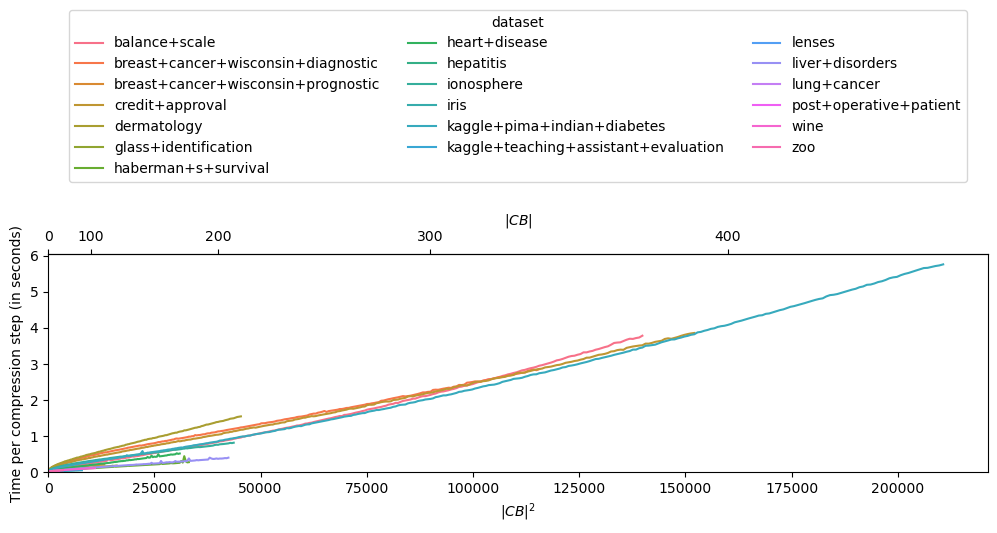
\includegraphics[width=\textwidth]{../results-no-sim-tuning+/figs/runtime-square.png}
    
\end{frame}

\section{Results on each dataset}

\begin{frame}{Metrics}

    Compression step: $step_i: |CB_i| = |CB_0| - i$

    ~

    Position and value for the maximum accuracy for all models
    
    \textit{if multiple with same score, take the one with the smallest CB}
\end{frame}

\begin{frame}{Result: Lenses}
    \begin{columns}
        \begin{column}{.3\textwidth}
            {\smaller\smaller\smaller
            \underline{\textbf{Lenses}} \\
            \textbf{Credit Approval} \\
            Zoo \\
            Wine \\
            Teaching Assistant Evaluation \\
            Post-Operative Patient \\
            Pima indians Diabetes \\
            Lung Cancer \\
            Liver Disorders \\
            Iris \\
            Ionosphere \\
            Hepatitis \\
            Heart Disease Cleveland \\
            Haberman's Survival \\
            Glass Identification \\
            Dermatology \\
            Breast Cancer Pronostic \\
            Breast Cancer Diagnostic \\
            Balance\\
            ~}
        \end{column}
        \begin{column}{.7\textwidth}
            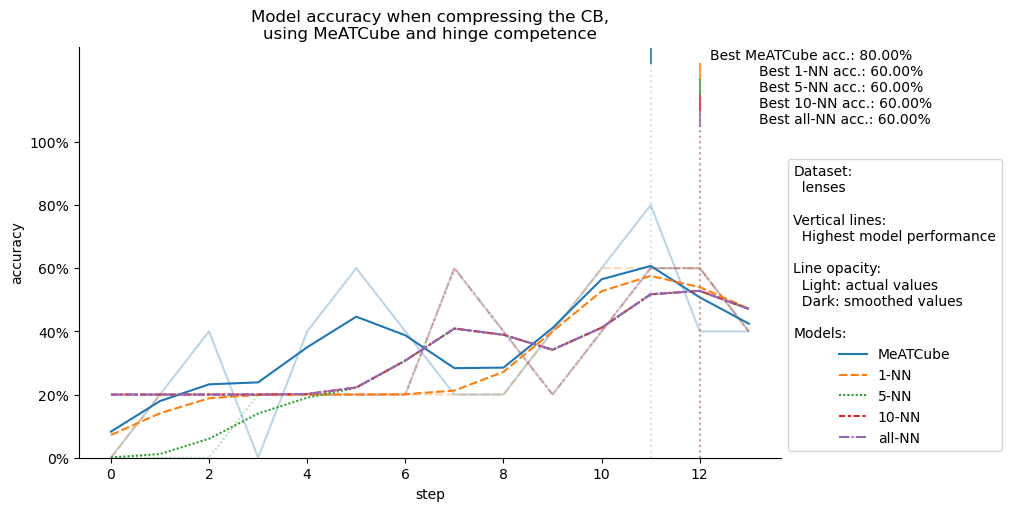
\includegraphics[width=\textwidth]{../results-no-sim-tuning+/figs/lenses}
            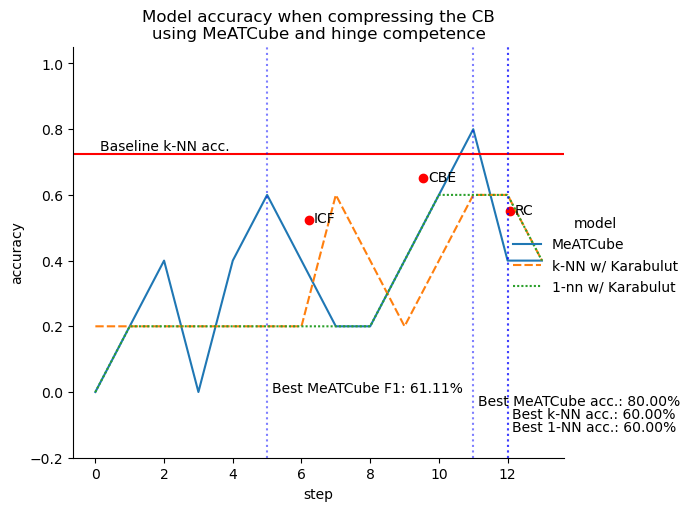
\includegraphics[width=.8\textwidth]{../obselete\_results/results-weight-estim+/figs/lenses}
        \end{column}
    \end{columns}
\end{frame}
\begin{frame}{Result: Credit Aproval}
    \begin{columns}
        \begin{column}{.3\textwidth}
            {\smaller\smaller\smaller
            \textbf{Lenses} \\
            \underline{\textbf{Credit Approval}} \\
            Zoo \\
            Wine \\
            Teaching Assistant Evaluation \\
            Post-Operative Patient \\
            Pima indians Diabetes \\
            Lung Cancer \\
            Liver Disorders \\
            Iris \\
            Ionosphere \\
            Hepatitis \\
            Heart Disease Cleveland \\
            Haberman's Survival \\
            Glass Identification \\
            Dermatology \\
            Breast Cancer Pronostic \\
            Breast Cancer Diagnostic \\
            Balance\\
            ~}
        \end{column}
        \begin{column}{.7\textwidth}
            \includegraphics[width=\textwidth]{../results-no-sim-tuning+/figs/credit+approval}
            \includegraphics[width=.8\textwidth]{../obselete\_results/results-weight-estim+/figs/credit+approval}
        \end{column}
    \end{columns}
\end{frame}
\begin{frame}{Result: Zoo}
    \begin{columns}
        \begin{column}{.3\textwidth}
            {\smaller\smaller\smaller
            \textbf{Lenses} \\
            \textbf{Credit Approval} \\
            \underline{Zoo} \\
            Wine \\
            Teaching Assistant Evaluation \\
            Post-Operative Patient \\
            Pima indians Diabetes \\
            Lung Cancer \\
            Liver Disorders \\
            Iris \\
            Ionosphere \\
            Hepatitis \\
            Heart Disease Cleveland \\
            Haberman's Survival \\
            Glass Identification \\
            Dermatology \\
            Breast Cancer Pronostic \\
            Breast Cancer Diagnostic \\
            Balance\\
            ~}
        \end{column}
        \begin{column}{.7\textwidth}
            \includegraphics[width=\textwidth]{../results-no-sim-tuning+/figs/zoo}
            \includegraphics[width=.8\textwidth]{../obselete\_results/results-weight-estim+/figs/zoo}
        \end{column}
    \end{columns}
\end{frame}
\begin{frame}{Result: Wine}
    \begin{columns}
        \begin{column}{.3\textwidth}
            {\smaller\smaller\smaller
            \textbf{Lenses} \\
            \textbf{Credit Approval} \\
            Zoo \\
            \underline{Wine} \\
            Teaching Assistant Evaluation \\
            Post-Operative Patient \\
            Pima indians Diabetes \\
            Lung Cancer \\
            Liver Disorders \\
            Iris \\
            Ionosphere \\
            Hepatitis \\
            Heart Disease Cleveland \\
            Haberman's Survival \\
            Glass Identification \\
            Dermatology \\
            Breast Cancer Pronostic \\
            Breast Cancer Diagnostic \\
            Balance\\
            ~}
        \end{column}
        \begin{column}{.7\textwidth}
            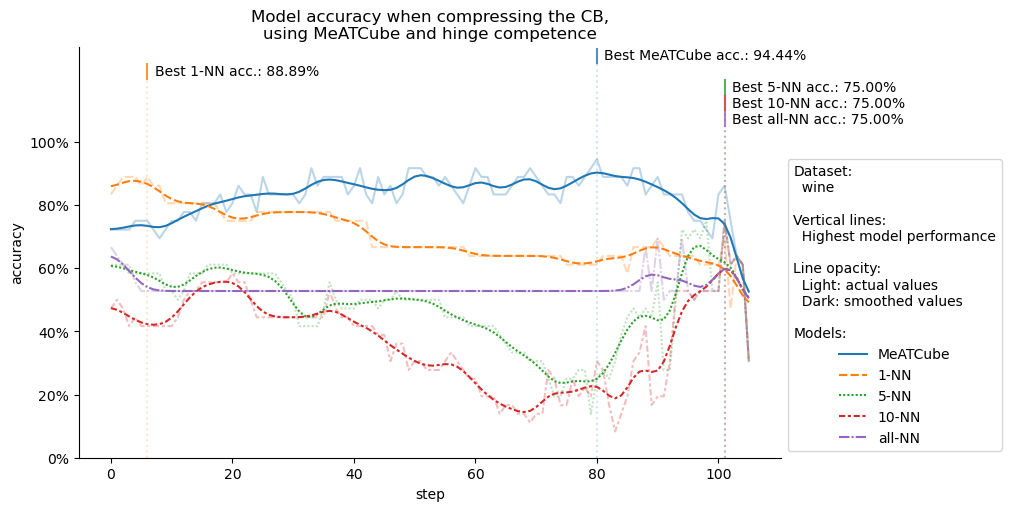
\includegraphics[width=\textwidth]{../results-no-sim-tuning+/figs/wine}
            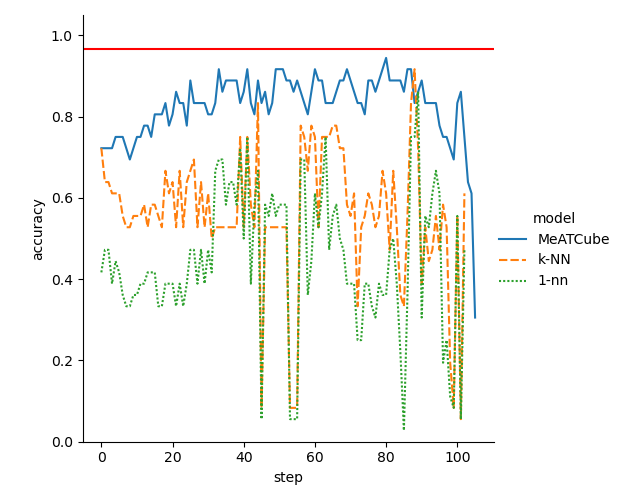
\includegraphics[width=.8\textwidth]{../obselete\_results/results-weight-estim+/figs/wine}
        \end{column}
    \end{columns}
\end{frame}
\begin{frame}{Result: Teach. Aassistant}
    \begin{columns}
        \begin{column}{.3\textwidth}
            {\smaller\smaller\smaller
            \textbf{Lenses} \\
            \textbf{Credit Approval} \\
            Zoo \\
            Wine \\
            \underline{Teaching Assistant Evaluation} \\
            Post-Operative Patient \\
            Pima indians Diabetes \\
            Lung Cancer \\
            Liver Disorders \\
            Iris \\
            Ionosphere \\
            Hepatitis \\
            Heart Disease Cleveland \\
            Haberman's Survival \\
            Glass Identification \\
            Dermatology \\
            Breast Cancer Pronostic \\
            Breast Cancer Diagnostic \\
            Balance\\
            ~}
        \end{column}
        \begin{column}{.7\textwidth}
            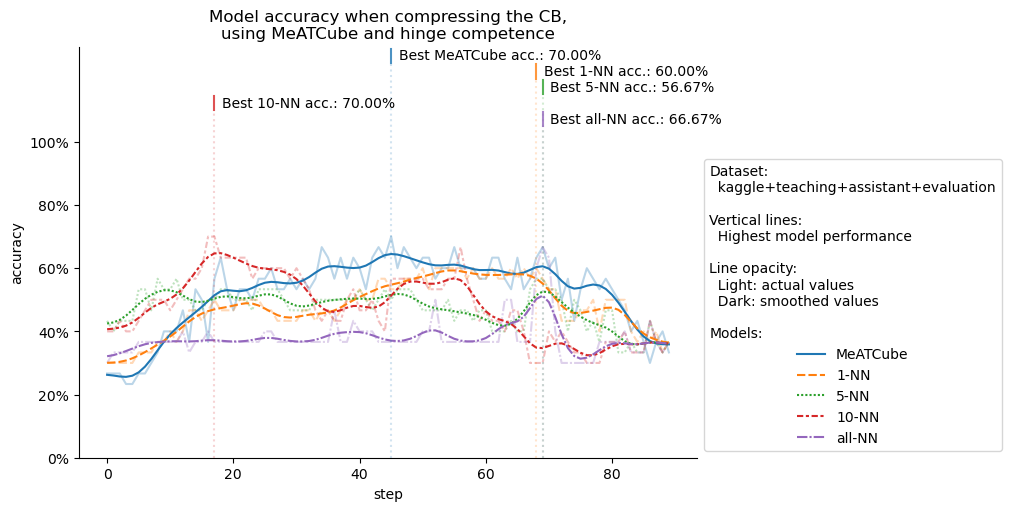
\includegraphics[width=\textwidth]{../results-no-sim-tuning+/figs/kaggle+teaching+assistant+evaluation.png}
            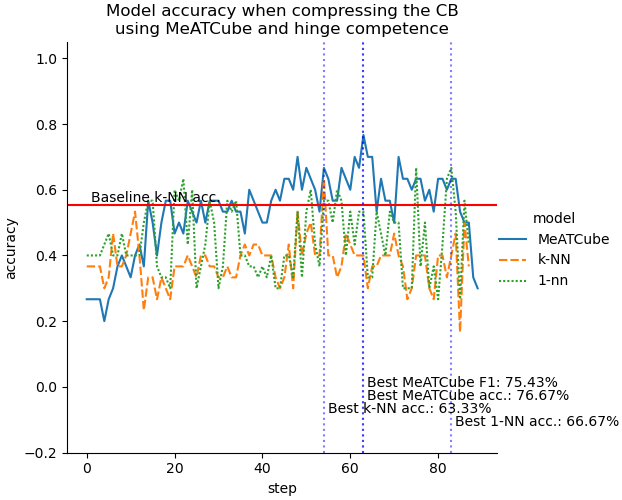
\includegraphics[width=.8\textwidth]{../obselete\_results/results-weight-estim+/figs/kaggle+teaching+assistant+evaluation.png}
        \end{column}
    \end{columns}
\end{frame}
\begin{frame}{Result: Post-Op. Patient}
    \begin{columns}
        \begin{column}{.3\textwidth}
            {\smaller\smaller\smaller
            \textbf{Lenses} \\
            \textbf{Credit Approval} \\
            Zoo \\
            Wine \\
            Teaching Assistant Evaluation \\
            \underline{Post-Operative Patient} \\
            Pima indians Diabetes \\
            Lung Cancer \\
            Liver Disorders \\
            Iris \\
            Ionosphere \\
            Hepatitis \\
            Heart Disease Cleveland \\
            Haberman's Survival \\
            Glass Identification \\
            Dermatology \\
            Breast Cancer Pronostic \\
            Breast Cancer Diagnostic \\
            Balance\\
            ~}
        \end{column}
        \begin{column}{.7\textwidth}
            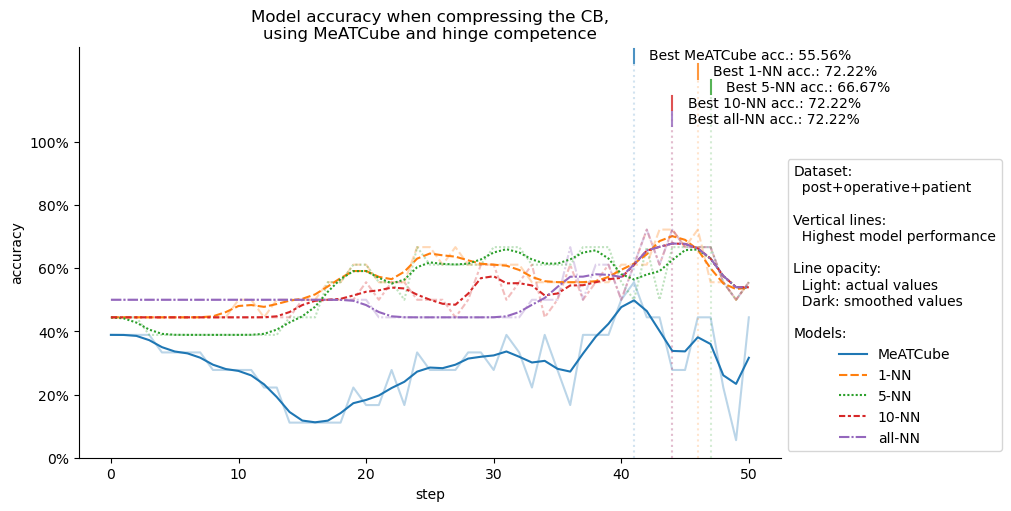
\includegraphics[width=\textwidth]{../results-no-sim-tuning+/figs/post+operative+patient.png}
            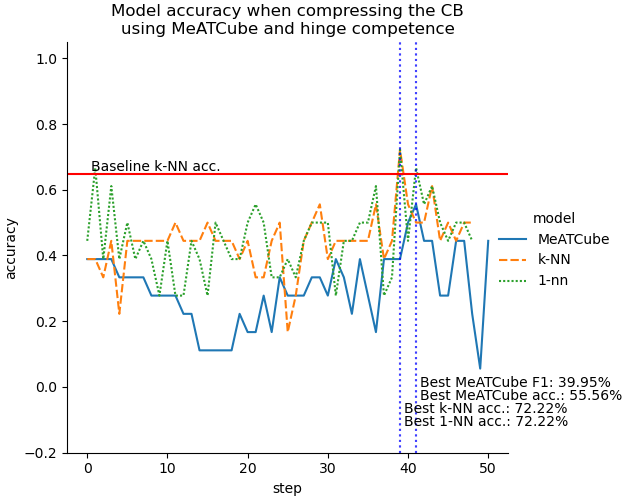
\includegraphics[width=.8\textwidth]{../obselete\_results/results-weight-estim+/figs/post+operative+patient.png}
        \end{column}
    \end{columns}
\end{frame}
\begin{frame}{Result: Pima}
    \begin{columns}
        \begin{column}{.3\textwidth}
            {\smaller\smaller\smaller
            \textbf{Lenses} \\
            \textbf{Credit Approval} \\
            Zoo \\
            Wine \\
            Teaching Assistant Evaluation \\
            Post-Operative Patient \\
            \underline{Pima indians Diabetes} \\
            Lung Cancer \\
            Liver Disorders \\
            Iris \\
            Ionosphere \\
            Hepatitis \\
            Heart Disease Cleveland \\
            Haberman's Survival \\
            Glass Identification \\
            Dermatology \\
            Breast Cancer Pronostic \\
            Breast Cancer Diagnostic \\
            Balance\\
            ~}
        \end{column}
        \begin{column}{.7\textwidth}
            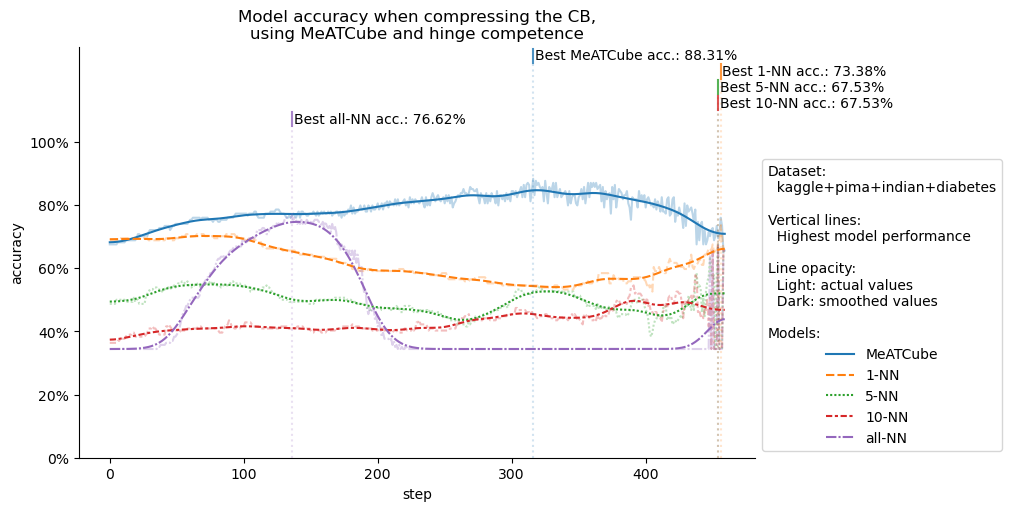
\includegraphics[width=\textwidth]{../results-no-sim-tuning+/figs/kaggle+pima+indian+diabetes.png}
            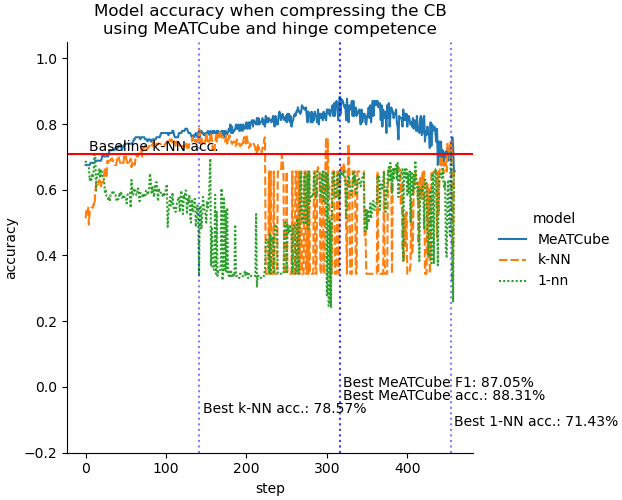
\includegraphics[width=.8\textwidth]{../obselete\_results/results-weight-estim+/figs/kaggle+pima+indian+diabetes.png}
        \end{column}
    \end{columns}
\end{frame}
\begin{frame}{Result: Lung Cancer}
    \begin{columns}
        \begin{column}{.3\textwidth}
            {\smaller\smaller\smaller
            \textbf{Lenses} \\
            \textbf{Credit Approval} \\
            Zoo \\
            Wine \\
            Teaching Assistant Evaluation \\
            Post-Operative Patient \\
            Pima indians Diabetes \\
            \underline{Lung Cancer} \\
            Liver Disorders \\
            Iris \\
            Ionosphere \\
            Hepatitis \\
            Heart Disease Cleveland \\
            Haberman's Survival \\
            Glass Identification \\
            Dermatology \\
            Breast Cancer Pronostic \\
            Breast Cancer Diagnostic \\
            Balance\\
            ~}
        \end{column}
        \begin{column}{.7\textwidth}
            \includegraphics[width=\textwidth]{../results-no-sim-tuning+/figs/lung+cancer.png}
            \includegraphics[width=.8\textwidth]{../obselete\_results/results-weight-estim+/figs/lung+cancer.png}
        \end{column}
    \end{columns}
\end{frame}
\begin{frame}{Result: Liver Disorders}
    \begin{columns}
        \begin{column}{.3\textwidth}
            {\smaller\smaller\smaller
            \textbf{Lenses} \\
            \textbf{Credit Approval} \\
            Zoo \\
            Wine \\
            Teaching Assistant Evaluation \\
            Post-Operative Patient \\
            Pima indians Diabetes \\
            Lung Cancer \\
            \underline{Liver Disorders} \\
            Iris \\
            Ionosphere \\
            Hepatitis \\
            Heart Disease Cleveland \\
            Haberman's Survival \\
            Glass Identification \\
            Dermatology \\
            Breast Cancer Pronostic \\
            Breast Cancer Diagnostic \\
            Balance\\
            ~}
        \end{column}
        \begin{column}{.7\textwidth}
            \includegraphics[width=\textwidth]{../results-no-sim-tuning+/figs/liver+disorders.png}
            \includegraphics[width=.8\textwidth]{../obselete\_results/results-weight-estim+/figs/liver+disorders.png}
        \end{column}
    \end{columns}
\end{frame}
\begin{frame}{Result: Iris}
    \begin{columns}
        \begin{column}{.3\textwidth}
            {\smaller\smaller\smaller
            \textbf{Lenses} \\
            \textbf{Credit Approval} \\
            Zoo \\
            Wine \\
            Teaching Assistant Evaluation \\
            Post-Operative Patient \\
            Pima indians Diabetes \\
            Lung Cancer \\
            Liver Disorders \\
            \underline{Iris} \\
            Ionosphere \\
            Hepatitis \\
            Heart Disease Cleveland \\
            Haberman's Survival \\
            Glass Identification \\
            Dermatology \\
            Breast Cancer Pronostic \\
            Breast Cancer Diagnostic \\
            Balance\\
            ~}
        \end{column}
        \begin{column}{.7\textwidth}
            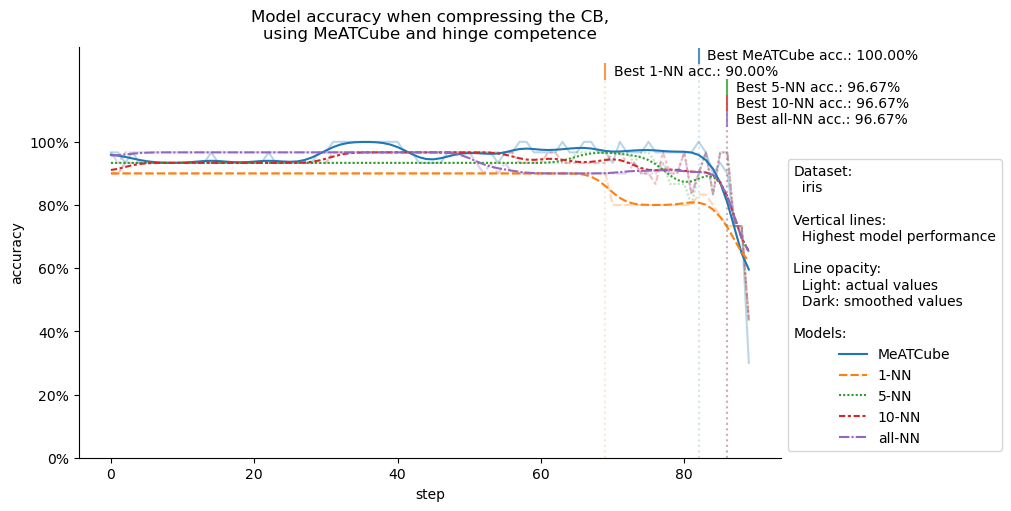
\includegraphics[width=\textwidth]{../results-no-sim-tuning+/figs/iris.png}
            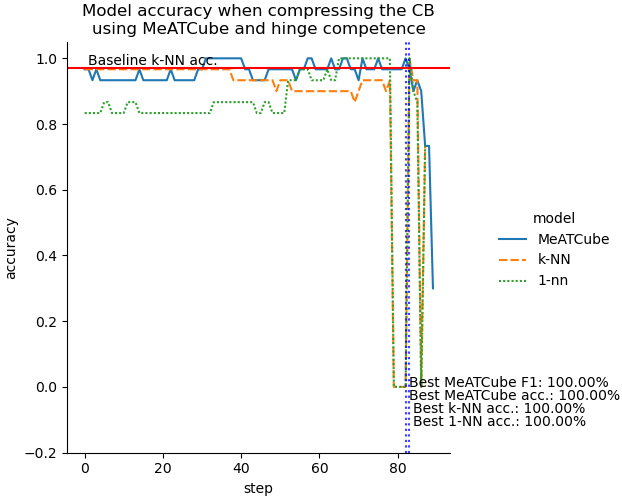
\includegraphics[width=.8\textwidth]{../obselete\_results/results-weight-estim+/figs/iris.png}
        \end{column}
    \end{columns}
\end{frame}
\begin{frame}{Result: Ionosphere}
    \begin{columns}
        \begin{column}{.3\textwidth}
            {\smaller\smaller\smaller
            \textbf{Lenses} \\
            \textbf{Credit Approval} \\
            Zoo \\
            Wine \\
            Teaching Assistant Evaluation \\
            Post-Operative Patient \\
            Pima indians Diabetes \\
            Lung Cancer \\
            Liver Disorders \\
            Iris \\
            \underline{Ionosphere} \\
            Hepatitis \\
            Heart Disease Cleveland \\
            Haberman's Survival \\
            Glass Identification \\
            Dermatology \\
            Breast Cancer Pronostic \\
            Breast Cancer Diagnostic \\
            Balance\\
            ~}
        \end{column}
        \begin{column}{.7\textwidth}
            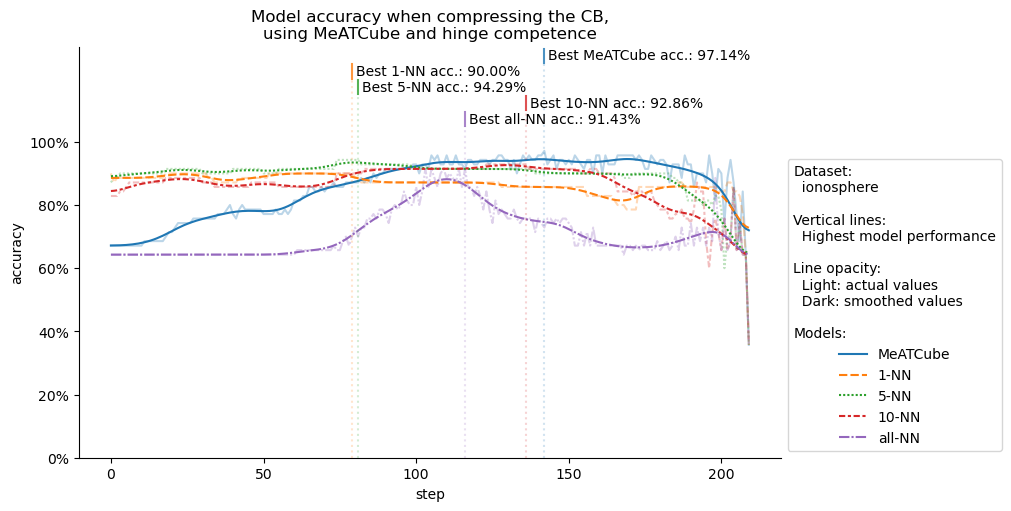
\includegraphics[width=\textwidth]{../results-no-sim-tuning+/figs/ionosphere.png}
            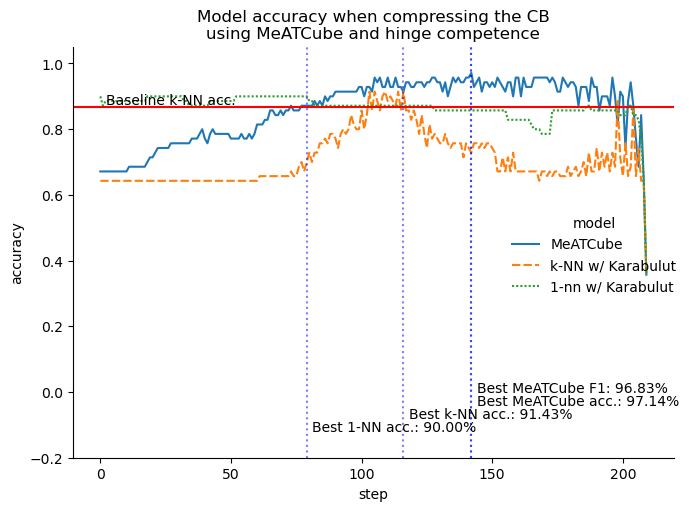
\includegraphics[width=.8\textwidth]{../obselete\_results/results-weight-estim+/figs/ionosphere.png}
        \end{column}
    \end{columns}
\end{frame}
\begin{frame}{Result: Hepatitis}
    \begin{columns}
        \begin{column}{.3\textwidth}
            {\smaller\smaller\smaller
            \textbf{Lenses} \\
            \textbf{Credit Approval} \\
            Zoo \\
            Wine \\
            Teaching Assistant Evaluation \\
            Post-Operative Patient \\
            Pima indians Diabetes \\
            Lung Cancer \\
            Liver Disorders \\
            Iris \\
            Ionosphere \\
            \underline{Hepatitis} \\
            Heart Disease Cleveland \\
            Haberman's Survival \\
            Glass Identification \\
            Dermatology \\
            Breast Cancer Pronostic \\
            Breast Cancer Diagnostic \\
            Balance\\
            ~}
        \end{column}
        \begin{column}{.7\textwidth}
            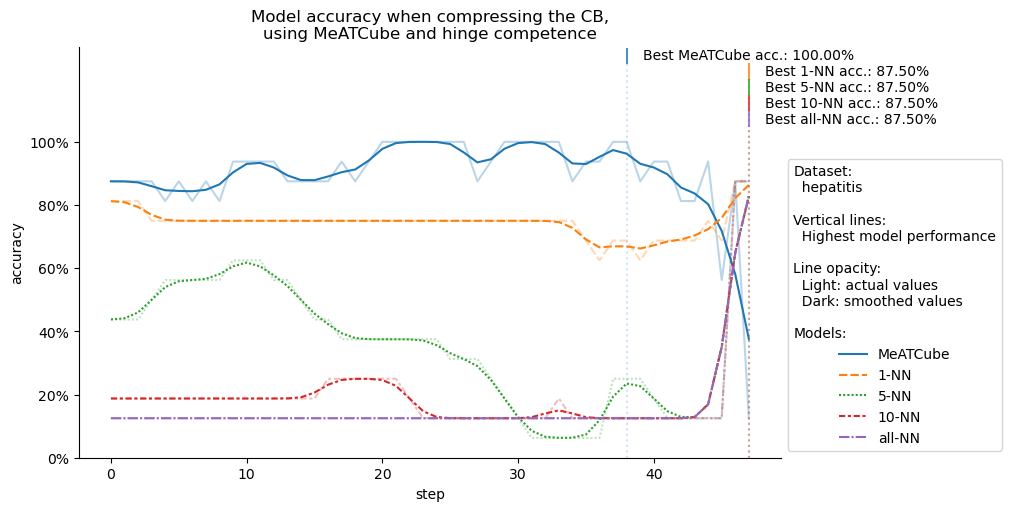
\includegraphics[width=\textwidth]{../results-no-sim-tuning+/figs/hepatitis.png}
            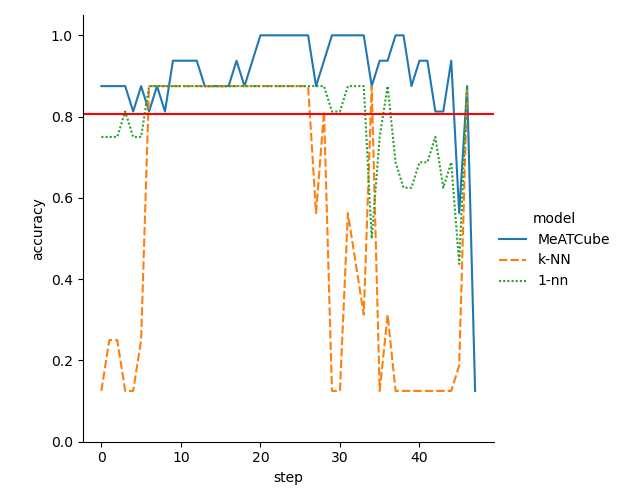
\includegraphics[width=.8\textwidth]{../obselete\_results/results-weight-estim+/figs/hepatitis.png}
        \end{column}
    \end{columns}
\end{frame}
\begin{frame}{Result: Heart}
    \begin{columns}
        \begin{column}{.3\textwidth}
            {\smaller\smaller\smaller
            \textbf{Lenses} \\
            \textbf{Credit Approval} \\
            Zoo \\
            Wine \\
            Teaching Assistant Evaluation \\
            Post-Operative Patient \\
            Pima indians Diabetes \\
            Lung Cancer \\
            Liver Disorders \\
            Iris \\
            Ionosphere \\
            Hepatitis \\
            \underline{Heart Disease Cleveland} \\
            Haberman's Survival \\
            Glass Identification \\
            Dermatology \\
            Breast Cancer Pronostic \\
            Breast Cancer Diagnostic \\
            Balance\\
            ~}
        \end{column}
        \begin{column}{.7\textwidth}
            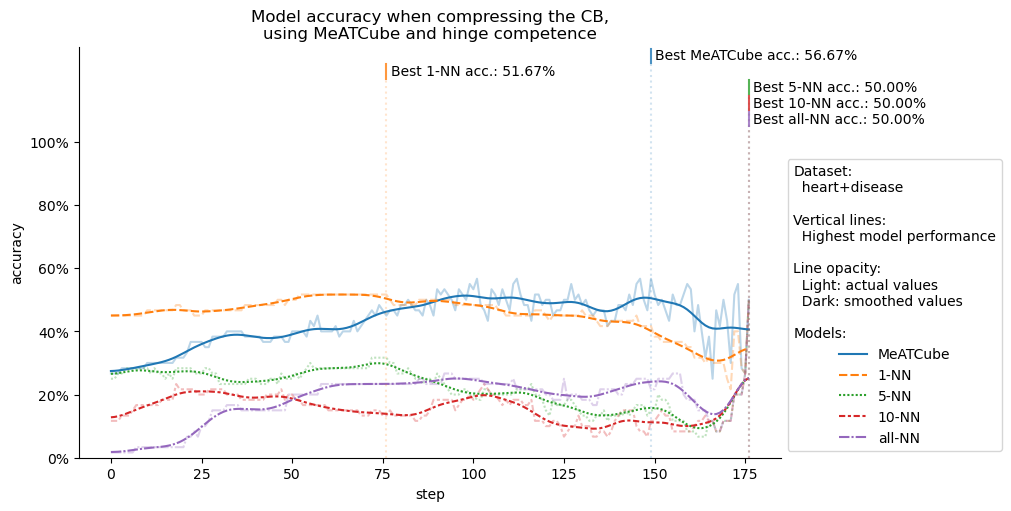
\includegraphics[width=\textwidth]{../results-no-sim-tuning+/figs/heart+disease.png}
            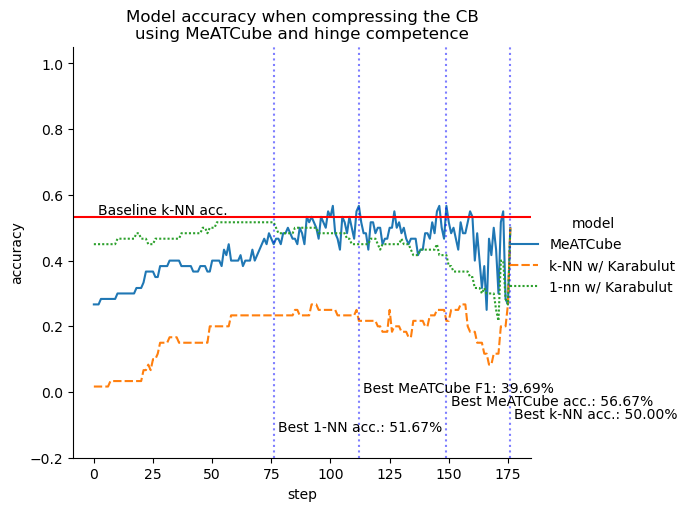
\includegraphics[width=.8\textwidth]{../obselete\_results/results-weight-estim+/figs/heart+disease.png}
        \end{column}
    \end{columns}
\end{frame}
\begin{frame}{Result: Haberman's}
    \begin{columns}
        \begin{column}{.3\textwidth}
            {\smaller\smaller\smaller
            \textbf{Lenses} \\
            \textbf{Credit Approval} \\
            Zoo \\
            Wine \\
            Teaching Assistant Evaluation \\
            Post-Operative Patient \\
            Pima indians Diabetes \\
            Lung Cancer \\
            Liver Disorders \\
            Iris \\
            Ionosphere \\
            Hepatitis \\
            Heart Disease Cleveland \\
            \underline{Haberman's Survival} \\
            Glass Identification \\
            Dermatology \\
            Breast Cancer Pronostic \\
            Breast Cancer Diagnostic \\
            Balance\\
            ~}
        \end{column}
        \begin{column}{.7\textwidth}
            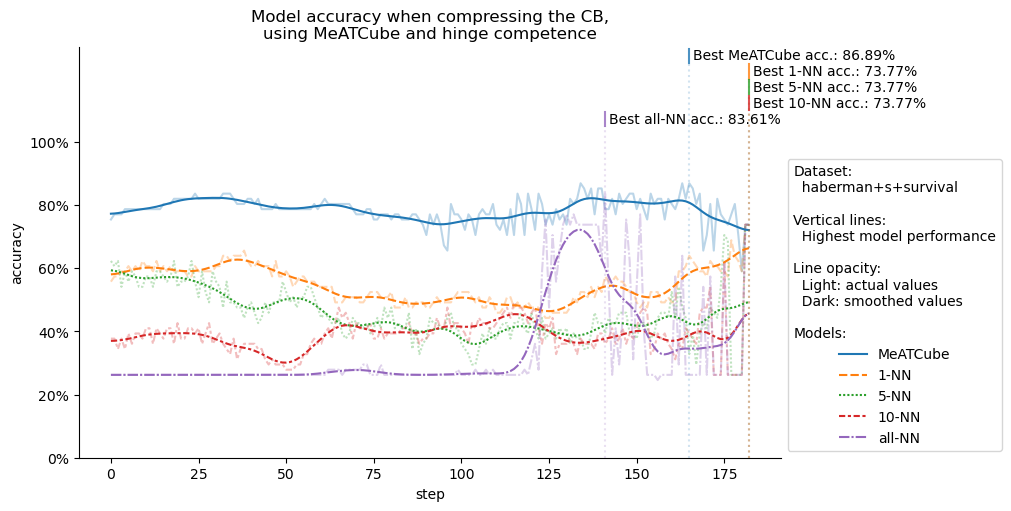
\includegraphics[width=\textwidth]{../results-no-sim-tuning+/figs/haberman+s+survival.png}
            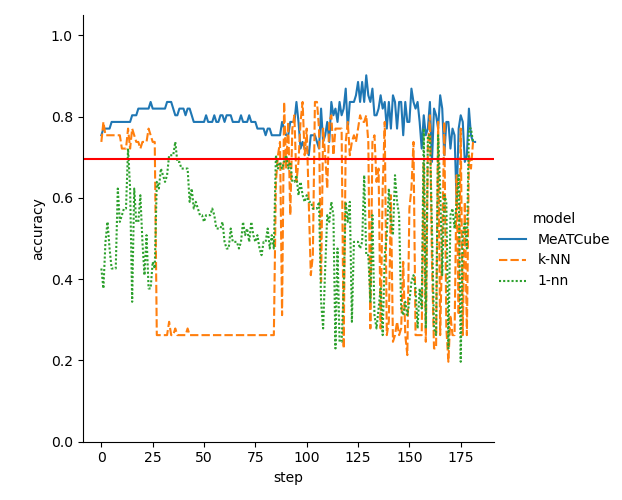
\includegraphics[width=.8\textwidth]{../obselete\_results/results-weight-estim+/figs/haberman+s+survival.png}
        \end{column}
    \end{columns}
\end{frame}
\begin{frame}{Result: Glass}
    \begin{columns}
        \begin{column}{.3\textwidth}
            {\smaller\smaller\smaller
            \textbf{Lenses} \\
            \textbf{Credit Approval} \\
            Zoo \\
            Wine \\
            Teaching Assistant Evaluation \\
            Post-Operative Patient \\
            Pima indians Diabetes \\
            Lung Cancer \\
            Liver Disorders \\
            Iris \\
            Ionosphere \\
            Hepatitis \\
            Heart Disease Cleveland \\
            Haberman's Survival \\
            \underline{Glass Identification} \\
            Dermatology \\
            Breast Cancer Pronostic \\
            Breast Cancer Diagnostic \\
            Balance\\
            ~}
        \end{column}
        \begin{column}{.7\textwidth}
            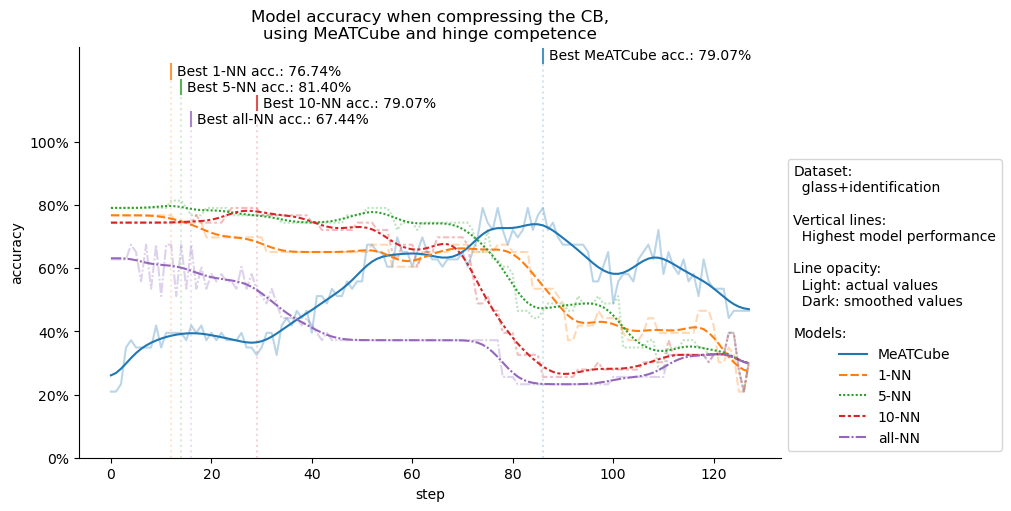
\includegraphics[width=\textwidth]{../results-no-sim-tuning+/figs/glass+identification.png}
            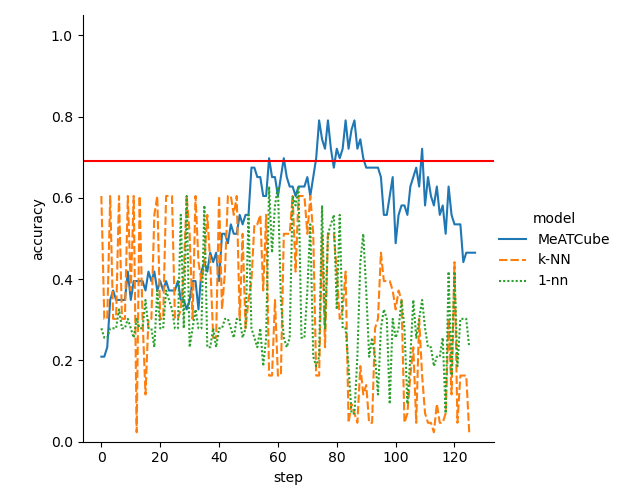
\includegraphics[width=.8\textwidth]{../obselete\_results/results-weight-estim+/figs/glass+identification.png}
        \end{column}
    \end{columns}
\end{frame}
\begin{frame}{Result: Dermatology}
    \begin{columns}
        \begin{column}{.3\textwidth}
            {\smaller\smaller\smaller
            \textbf{Lenses} \\
            \textbf{Credit Approval} \\
            Zoo \\
            Wine \\
            Teaching Assistant Evaluation \\
            Post-Operative Patient \\
            Pima indians Diabetes \\
            Lung Cancer \\
            Liver Disorders \\
            Iris \\
            Ionosphere \\
            Hepatitis \\
            Heart Disease Cleveland \\
            Haberman's Survival \\
            Glass Identification \\
            \underline{Dermatology} \\
            Breast Cancer Pronostic \\
            Breast Cancer Diagnostic \\
            Balance\\
            ~}
        \end{column}
        \begin{column}{.7\textwidth}
            \includegraphics[width=\textwidth]{../results-no-sim-tuning+/figs/dermatology.png}
            \includegraphics[width=.8\textwidth]{../obselete\_results/results-weight-estim+/figs/dermatology.png}
        \end{column}
    \end{columns}
\end{frame}
\begin{frame}{Result: Breast Cancer Pronostic}
    \begin{columns}
        \begin{column}{.3\textwidth}
            {\smaller\smaller\smaller
            \textbf{Lenses} \\
            \textbf{Credit Approval} \\
            Zoo \\
            Wine \\
            Teaching Assistant Evaluation \\
            Post-Operative Patient \\
            Pima indians Diabetes \\
            Lung Cancer \\
            Liver Disorders \\
            Iris \\
            Ionosphere \\
            Hepatitis \\
            Heart Disease Cleveland \\
            Haberman's Survival \\
            Glass Identification \\
            Dermatology \\
            \underline{Breast Cancer Pronostic} \\
            Breast Cancer Diagnostic \\
            Balance\\
            ~}
        \end{column}
        \begin{column}{.7\textwidth}
            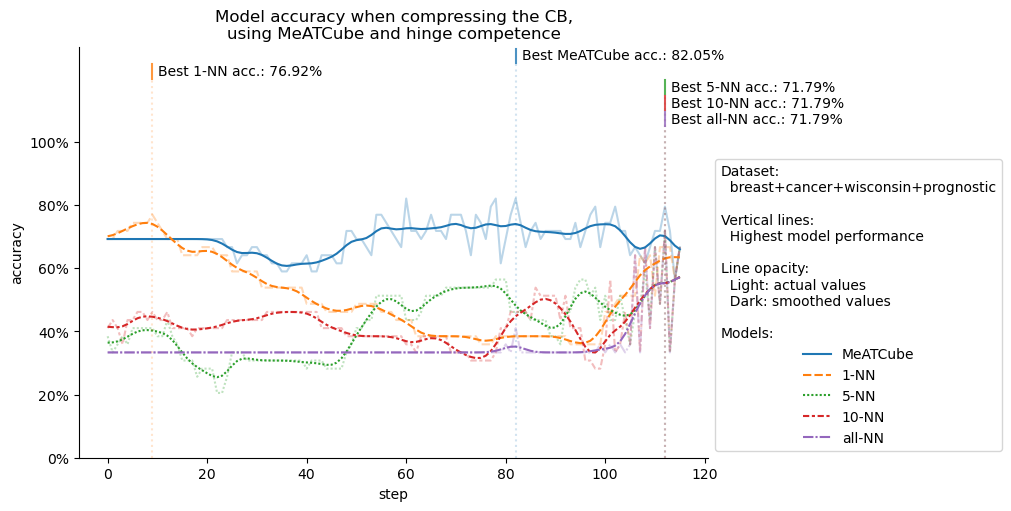
\includegraphics[width=\textwidth]{../results-no-sim-tuning+/figs/breast+cancer+wisconsin+prognostic.png}
            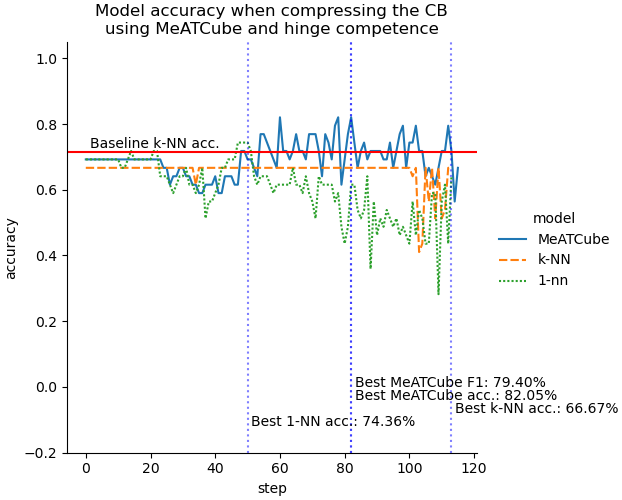
\includegraphics[width=.8\textwidth]{../obselete\_results/results-weight-estim+/figs/breast+cancer+wisconsin+prognostic.png}
        \end{column}
    \end{columns}
\end{frame}
\begin{frame}{Result: Breast Cancer Diagnostic}
    \begin{columns}
        \begin{column}{.3\textwidth}
            {\smaller\smaller\smaller
            \textbf{Lenses} \\
            \textbf{Credit Approval} \\
            Zoo \\
            Wine \\
            Teaching Assistant Evaluation \\
            Post-Operative Patient \\
            Pima indians Diabetes \\
            Lung Cancer \\
            Liver Disorders \\
            Iris \\
            Ionosphere \\
            Hepatitis \\
            Heart Disease Cleveland \\
            Haberman's Survival \\
            Glass Identification \\
            Dermatology \\
            Breast Cancer Pronostic \\
            \underline{Breast Cancer Diagnostic} \\
            Balance\\
            ~}
        \end{column}
        \begin{column}{.7\textwidth}
            \includegraphics[width=\textwidth]{../results-no-sim-tuning+/figs/breast+cancer+wisconsin+diagnostic.png}
            \includegraphics[width=.8\textwidth]{../obselete\_results/results-weight-estim+/figs/breast+cancer+wisconsin+diagnostic.png}
        \end{column}
    \end{columns}
\end{frame}
\begin{frame}{Result: Balance}
    \begin{columns}
        \begin{column}{.3\textwidth}
            {\smaller\smaller\smaller
            \textbf{Lenses} \\
            \textbf{Credit Approval} \\
            Zoo \\
            Wine \\
            Teaching Assistant Evaluation \\
            Post-Operative Patient \\
            Pima indians Diabetes \\
            Lung Cancer \\
            Liver Disorders \\
            Iris \\
            Ionosphere \\
            Hepatitis \\
            Heart Disease Cleveland \\
            Haberman's Survival \\
            Glass Identification \\
            Dermatology \\
            Breast Cancer Pronostic \\
            Breast Cancer Diagnostic \\
            \underline{Balance}\\
            ~}
        \end{column}
        \begin{column}{.7\textwidth}
            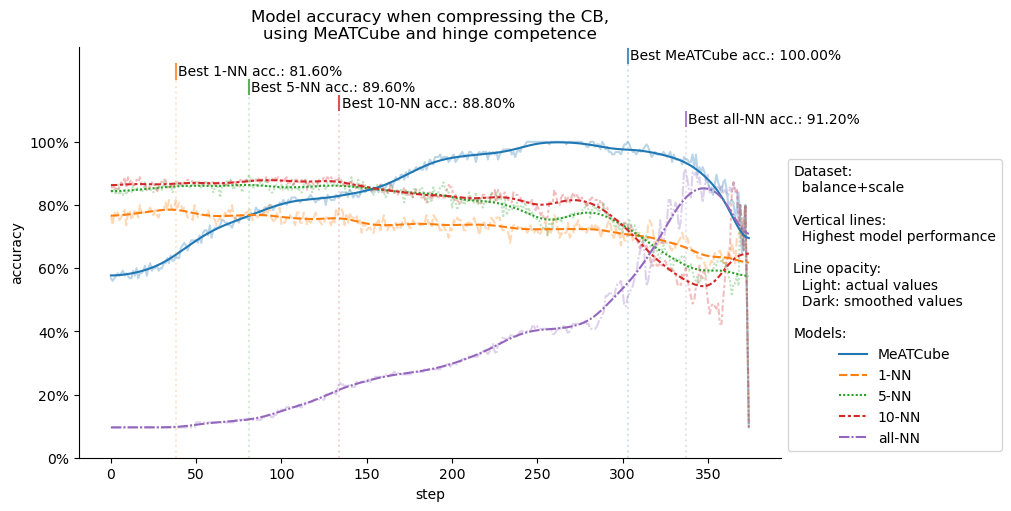
\includegraphics[width=\textwidth]{../results-no-sim-tuning+/figs/balance+scale}
            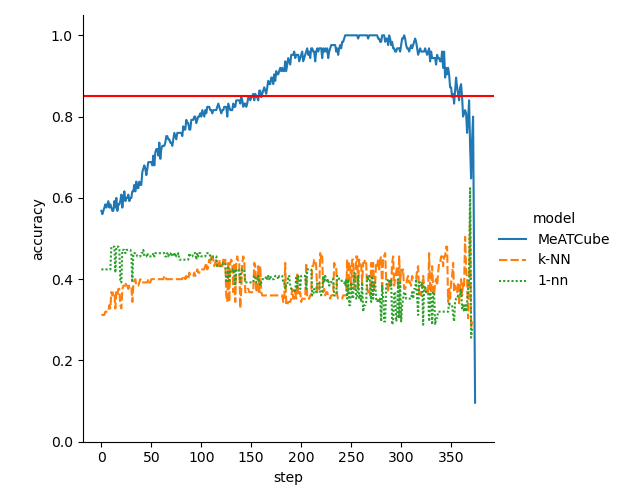
\includegraphics[width=.8\textwidth]{../obselete\_results/results-weight-estim+/figs/balance+scale}
        \end{column}
    \end{columns}
\end{frame}


\section{What next}
\begin{frame}{What next}
    Datasets to add?

    ~

    Fixing the weights: how?

    ~

    Apply the baselines instead of copying them

    Apply more recent baselines

    ~

    Cross-validation
\end{frame}
\end{document}